# SNAPSHOT_SOURCE: lindicaphxag-tech/cs@0b26a5b0853e3b136a92c17e614a3a1936673621 path=papers/eeg-default-regularisation/paper_vnext/93_figure_participant_effects.tex
% Auto-created only from immutable per-participant paired-effect vectors.
% Source GitHub blob SHA: 3f4d3fff3128ed4ddc95f2e392ae0acc48874d9b
% This is a supplementary DESCRIPTIVE figure; no new statistical test.
\begin{figure*}[t]
\centering
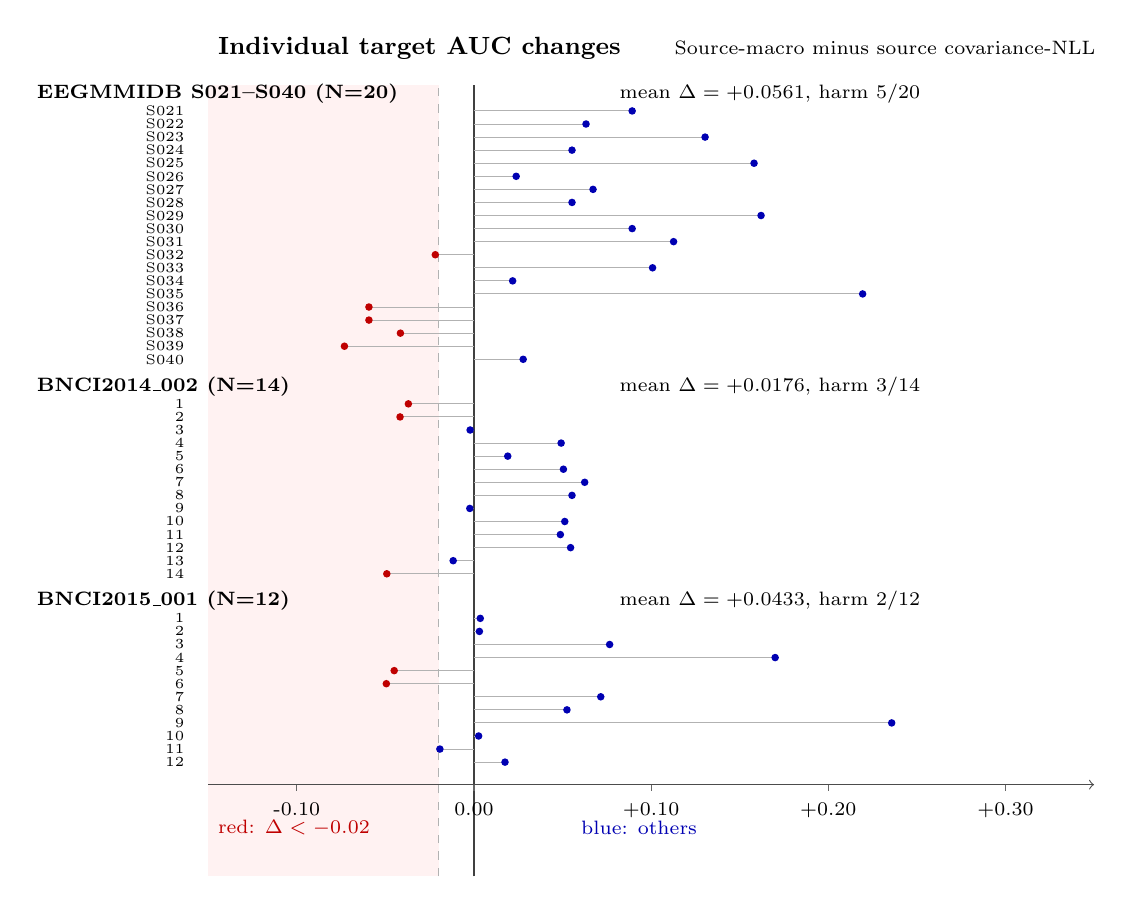
\begin{tikzpicture}[x=1cm,y=1cm]
\fill[red!5] (2.300,1.68) rectangle (5.225,11.73);
\draw[dashed, gray!60] (5.225,1.68) -- (5.225,11.73);
\draw[black!75,line width=0.55pt] (5.675,1.68) -- (5.675,11.73);
\node[anchor=west,font=\small\bfseries] at (2.3,12.2) {Individual target AUC changes};
\node[anchor=west,font=\scriptsize] at (8.1,12.2) {Source-macro minus source covariance-NLL};
\node[anchor=west,font=\scriptsize\bfseries] at (0.0,11.620) {EEGMMIDB S021--S040 (N=20)};
\node[anchor=west,font=\scriptsize] at (7.4,11.620) {mean $\Delta=+0.0561$, harm 5/20};
\node[anchor=east,font=\tiny] at (2.12,11.400) {S021};
\draw[black!30,line width=0.35pt] (5.675,11.400) -- (7.684,11.400);
\fill[blue!70!black] (7.684,11.400) circle (0.048);
\node[anchor=east,font=\tiny] at (2.12,11.234) {S022};
\draw[black!30,line width=0.35pt] (5.675,11.234) -- (7.098,11.234);
\fill[blue!70!black] (7.098,11.234) circle (0.048);
\node[anchor=east,font=\tiny] at (2.12,11.068) {S023};
\draw[black!30,line width=0.35pt] (5.675,11.068) -- (8.610,11.068);
\fill[blue!70!black] (8.610,11.068) circle (0.048);
\node[anchor=east,font=\tiny] at (2.12,10.902) {S024};
\draw[black!30,line width=0.35pt] (5.675,10.902) -- (6.920,10.902);
\fill[blue!70!black] (6.920,10.902) circle (0.048);
\node[anchor=east,font=\tiny] at (2.12,10.736) {S025};
\draw[black!30,line width=0.35pt] (5.675,10.736) -- (9.232,10.736);
\fill[blue!70!black] (9.232,10.736) circle (0.048);
\node[anchor=east,font=\tiny] at (2.12,10.570) {S026};
\draw[black!30,line width=0.35pt] (5.675,10.570) -- (6.211,10.570);
\fill[blue!70!black] (6.211,10.570) circle (0.048);
\node[anchor=east,font=\tiny] at (2.12,10.404) {S027};
\draw[black!30,line width=0.35pt] (5.675,10.404) -- (7.187,10.404);
\fill[blue!70!black] (7.187,10.404) circle (0.048);
\node[anchor=east,font=\tiny] at (2.12,10.238) {S028};
\draw[black!30,line width=0.35pt] (5.675,10.238) -- (6.920,10.238);
\fill[blue!70!black] (6.920,10.238) circle (0.048);
\node[anchor=east,font=\tiny] at (2.12,10.072) {S029};
\draw[black!30,line width=0.35pt] (5.675,10.072) -- (9.321,10.072);
\fill[blue!70!black] (9.321,10.072) circle (0.048);
\node[anchor=east,font=\tiny] at (2.12,9.906) {S030};
\draw[black!30,line width=0.35pt] (5.675,9.906) -- (7.684,9.906);
\fill[blue!70!black] (7.684,9.906) circle (0.048);
\node[anchor=east,font=\tiny] at (2.12,9.740) {S031};
\draw[black!30,line width=0.35pt] (5.675,9.740) -- (8.210,9.740);
\fill[blue!70!black] (8.210,9.740) circle (0.048);
\node[anchor=east,font=\tiny] at (2.12,9.574) {S032};
\draw[black!30,line width=0.35pt] (5.675,9.574) -- (5.184,9.574);
\fill[red!75!black] (5.184,9.574) circle (0.048);
\node[anchor=east,font=\tiny] at (2.12,9.408) {S033};
\draw[black!30,line width=0.35pt] (5.675,9.408) -- (7.943,9.408);
\fill[blue!70!black] (7.943,9.408) circle (0.048);
\node[anchor=east,font=\tiny] at (2.12,9.242) {S034};
\draw[black!30,line width=0.35pt] (5.675,9.242) -- (6.166,9.242);
\fill[blue!70!black] (6.166,9.242) circle (0.048);
\node[anchor=east,font=\tiny] at (2.12,9.076) {S035};
\draw[black!30,line width=0.35pt] (5.675,9.076) -- (10.611,9.076);
\fill[blue!70!black] (10.611,9.076) circle (0.048);
\node[anchor=east,font=\tiny] at (2.12,8.910) {S036};
\draw[black!30,line width=0.35pt] (5.675,8.910) -- (4.341,8.910);
\fill[red!75!black] (4.341,8.910) circle (0.048);
\node[anchor=east,font=\tiny] at (2.12,8.744) {S037};
\draw[black!30,line width=0.35pt] (5.675,8.744) -- (4.341,8.744);
\fill[red!75!black] (4.341,8.744) circle (0.048);
\node[anchor=east,font=\tiny] at (2.12,8.578) {S038};
\draw[black!30,line width=0.35pt] (5.675,8.578) -- (4.741,8.578);
\fill[red!75!black] (4.741,8.578) circle (0.048);
\node[anchor=east,font=\tiny] at (2.12,8.412) {S039};
\draw[black!30,line width=0.35pt] (5.675,8.412) -- (4.030,8.412);
\fill[red!75!black] (4.030,8.412) circle (0.048);
\node[anchor=east,font=\tiny] at (2.12,8.246) {S040};
\draw[black!30,line width=0.35pt] (5.675,8.246) -- (6.300,8.246);
\fill[blue!70!black] (6.300,8.246) circle (0.048);
\node[anchor=west,font=\scriptsize\bfseries] at (0.0,7.900) {BNCI2014\_002 (N=14)};
\node[anchor=west,font=\scriptsize] at (7.4,7.900) {mean $\Delta=+0.0176$, harm 3/14};
\node[anchor=east,font=\tiny] at (2.12,7.680) {1};
\draw[black!30,line width=0.35pt] (5.675,7.680) -- (4.842,7.680);
\fill[red!75!black] (4.842,7.680) circle (0.048);
\node[anchor=east,font=\tiny] at (2.12,7.514) {2};
\draw[black!30,line width=0.35pt] (5.675,7.514) -- (4.736,7.514);
\fill[red!75!black] (4.736,7.514) circle (0.048);
\node[anchor=east,font=\tiny] at (2.12,7.348) {3};
\draw[black!30,line width=0.35pt] (5.675,7.348) -- (5.626,7.348);
\fill[blue!70!black] (5.626,7.348) circle (0.048);
\node[anchor=east,font=\tiny] at (2.12,7.182) {4};
\draw[black!30,line width=0.35pt] (5.675,7.182) -- (6.782,7.182);
\fill[blue!70!black] (6.782,7.182) circle (0.048);
\node[anchor=east,font=\tiny] at (2.12,7.016) {5};
\draw[black!30,line width=0.35pt] (5.675,7.016) -- (6.104,7.016);
\fill[blue!70!black] (6.104,7.016) circle (0.048);
\node[anchor=east,font=\tiny] at (2.12,6.850) {6};
\draw[black!30,line width=0.35pt] (5.675,6.850) -- (6.811,6.850);
\fill[blue!70!black] (6.811,6.850) circle (0.048);
\node[anchor=east,font=\tiny] at (2.12,6.684) {7};
\draw[black!30,line width=0.35pt] (5.675,6.684) -- (7.081,6.684);
\fill[blue!70!black] (7.081,6.684) circle (0.048);
\node[anchor=east,font=\tiny] at (2.12,6.518) {8};
\draw[black!30,line width=0.35pt] (5.675,6.518) -- (6.920,6.518);
\fill[blue!70!black] (6.920,6.518) circle (0.048);
\node[anchor=east,font=\tiny] at (2.12,6.352) {9};
\draw[black!30,line width=0.35pt] (5.675,6.352) -- (5.622,6.352);
\fill[blue!70!black] (5.622,6.352) circle (0.048);
\node[anchor=east,font=\tiny] at (2.12,6.186) {10};
\draw[black!30,line width=0.35pt] (5.675,6.186) -- (6.828,6.186);
\fill[blue!70!black] (6.828,6.186) circle (0.048);
\node[anchor=east,font=\tiny] at (2.12,6.020) {11};
\draw[black!30,line width=0.35pt] (5.675,6.020) -- (6.772,6.020);
\fill[blue!70!black] (6.772,6.020) circle (0.048);
\node[anchor=east,font=\tiny] at (2.12,5.854) {12};
\draw[black!30,line width=0.35pt] (5.675,5.854) -- (6.902,5.854);
\fill[blue!70!black] (6.902,5.854) circle (0.048);
\node[anchor=east,font=\tiny] at (2.12,5.688) {13};
\draw[black!30,line width=0.35pt] (5.675,5.688) -- (5.411,5.688);
\fill[blue!70!black] (5.411,5.688) circle (0.048);
\node[anchor=east,font=\tiny] at (2.12,5.522) {14};
\draw[black!30,line width=0.35pt] (5.675,5.522) -- (4.568,5.522);
\fill[red!75!black] (4.568,5.522) circle (0.048);
\node[anchor=west,font=\scriptsize\bfseries] at (0.0,5.176) {BNCI2015\_001 (N=12)};
\node[anchor=west,font=\scriptsize] at (7.4,5.176) {mean $\Delta=+0.0433$, harm 2/12};
\node[anchor=east,font=\tiny] at (2.12,4.956) {1};
\draw[black!30,line width=0.35pt] (5.675,4.956) -- (5.755,4.956);
\fill[blue!70!black] (5.755,4.956) circle (0.048);
\node[anchor=east,font=\tiny] at (2.12,4.790) {2};
\draw[black!30,line width=0.35pt] (5.675,4.790) -- (5.744,4.790);
\fill[blue!70!black] (5.744,4.790) circle (0.048);
\node[anchor=east,font=\tiny] at (2.12,4.624) {3};
\draw[black!30,line width=0.35pt] (5.675,4.624) -- (7.398,4.624);
\fill[blue!70!black] (7.398,4.624) circle (0.048);
\node[anchor=east,font=\tiny] at (2.12,4.458) {4};
\draw[black!30,line width=0.35pt] (5.675,4.458) -- (9.500,4.458);
\fill[blue!70!black] (9.500,4.458) circle (0.048);
\node[anchor=east,font=\tiny] at (2.12,4.292) {5};
\draw[black!30,line width=0.35pt] (5.675,4.292) -- (4.662,4.292);
\fill[red!75!black] (4.662,4.292) circle (0.048);
\node[anchor=east,font=\tiny] at (2.12,4.126) {6};
\draw[black!30,line width=0.35pt] (5.675,4.126) -- (4.562,4.126);
\fill[red!75!black] (4.562,4.126) circle (0.048);
\node[anchor=east,font=\tiny] at (2.12,3.960) {7};
\draw[black!30,line width=0.35pt] (5.675,3.960) -- (7.285,3.960);
\fill[blue!70!black] (7.285,3.960) circle (0.048);
\node[anchor=east,font=\tiny] at (2.12,3.794) {8};
\draw[black!30,line width=0.35pt] (5.675,3.794) -- (6.856,3.794);
\fill[blue!70!black] (6.856,3.794) circle (0.048);
\node[anchor=east,font=\tiny] at (2.12,3.628) {9};
\draw[black!30,line width=0.35pt] (5.675,3.628) -- (10.980,3.628);
\fill[blue!70!black] (10.980,3.628) circle (0.048);
\node[anchor=east,font=\tiny] at (2.12,3.462) {10};
\draw[black!30,line width=0.35pt] (5.675,3.462) -- (5.734,3.462);
\fill[blue!70!black] (5.734,3.462) circle (0.048);
\node[anchor=east,font=\tiny] at (2.12,3.296) {11};
\draw[black!30,line width=0.35pt] (5.675,3.296) -- (5.242,3.296);
\fill[blue!70!black] (5.242,3.296) circle (0.048);
\node[anchor=east,font=\tiny] at (2.12,3.130) {12};
\draw[black!30,line width=0.35pt] (5.675,3.130) -- (6.069,3.130);
\fill[blue!70!black] (6.069,3.130) circle (0.048);
\draw[->,black!70] (2.300,2.844) -- (13.550,2.844);
\draw[black!60] (3.425,2.844) -- (3.425,2.764);
\node[anchor=north,font=\scriptsize] at (3.425,2.734) {-0.10};
\draw[black!60] (5.675,2.844) -- (5.675,2.764);
\node[anchor=north,font=\scriptsize] at (5.675,2.734) {0.00};
\draw[black!60] (7.925,2.844) -- (7.925,2.764);
\node[anchor=north,font=\scriptsize] at (7.925,2.734) {+0.10};
\draw[black!60] (10.175,2.844) -- (10.175,2.764);
\node[anchor=north,font=\scriptsize] at (10.175,2.734) {+0.20};
\draw[black!60] (12.425,2.844) -- (12.425,2.764);
\node[anchor=north,font=\scriptsize] at (12.425,2.734) {+0.30};
\node[anchor=west,font=\scriptsize,red!75!black] at (2.300,2.294) {red: $\Delta<-0.02$};
\node[anchor=west,font=\scriptsize,blue!70!black] at (6.912,2.294) {blue: others};
\end{tikzpicture}
\caption{Paired participant-level target AUC differences between the frozen source participant-macro selector and the source covariance-NLL selector in three EEG cohorts. Five of 20, three of 14 and two of 12 participants, respectively, lost more than 0.02 AUC. The vertical reference line is zero, and the tinted region denotes the material-harm threshold. EEGMMIDB was a prospectively frozen within-database block; both BNCI datasets were TRUE PRE-DATA external cohorts whose Holm-adjusted primary comparisons remain individually inconclusive. Points are descriptive and must not be treated as independent trials or a new confirmatory family.}
\label{fig:participant-harm-v10}
\end{figure*}
